\subsection{Image Zonal Anatomy Segmentation and 3D Model Rendering}
\subsubsection{MR Image Segmentation and Modeling}
Axial MR T2WI images were manually segmented using the smooth polygon tool in
ITK-SNAP~\cite{Yushkevich2006}, using unique labels for the PZ, CG and AFS. The
gland was segmented from base to apex.  The base was identified below the
bladder, and subsequent images were segmented until the last slice with visible
prostatic tissue was identified caudally. The CG and urethra, PZ and AFS were
segmented independently according to their well-established anatomical
characteristics on
T2WI.~\cite{Barentsz2012,Jung2012,Poon1985,Hricak2007,Bonekamp2011} The PZ was
identified by its homogenous high signal intensity on T2WI, which is usually
similar to that of the nearby periprostatic fat. The CG was visualized and
delineated based on its heterogeneous and lower signal intensity as well as its
location (Figure~\ref{fig:mr_anatomy}). The urethra was included in the CG
segmentation. Although not readily visible on every case, the AFS was
identified by its low T2 signal intensity and its location anterior to the
central gland. 

Segmented image stacks were imported into 3D Slicer (v4.3.0) and 3D
models were rendered using the following parameters (Table~\ref{tab:3dslicer}):

\begin{table}[h!]
\centering
\caption{3D model volume rendering parameters}
\begin{tabular}{ll}
{\bf Parameter} & {\bf Value} \\ \hline
Decimation & 0.1 \\
Smoothing Algorithm & Laplacian \\
Smoothing  & 70.0 \\
Joint Smoothing & Enabled \\
\end{tabular}
\label{tab:3dslicer}
\end{table}

The 3D models were used to render volume estimates of the PZ and CG, with the
sum of PZ and CG representing the total prostate gland volume. AFS volume
estimates in select MR cases were included in the total prostate gland volume
estimates. Orthogonal tri-axial measurements in the lateral-to-lateral,
apex-to-base, and anterior-to-posterior dimensions were made in slicer by
placing an ROI cube in the model's center and expanding the ROI cube to fit the
maximal model dimensions (Figure~\ref{fig:roi_tool}). 

Figure~\ref{fig:mr_anatomy} shows the anatomic zones and some anatomic
orientation labels in the prostate of a representative study subject MR T2WI.
The zonal anatomy of the prostate was manually segmented
(Figure~\ref{fig:mr_segs_vol}, bottom left) across the image stack, and 3D
models of the zonal anatomy volumes were rendered
(Figure~\ref{fig:mr_segs_vol}, top).

\begin{figure}
\centering
\begin{tabular}{ccc}
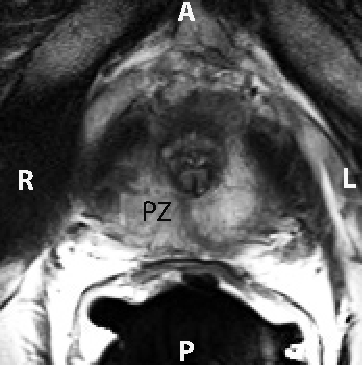
\includegraphics[width=0.29\linewidth]{figs/mr_anatomy/T2_apex} &
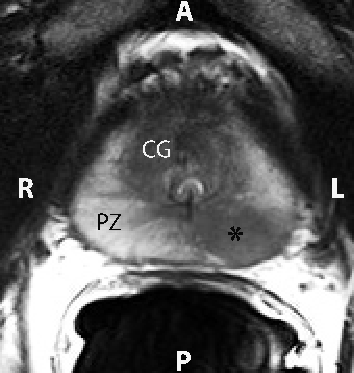
\includegraphics[width=0.275\linewidth]{figs/mr_anatomy/T2_midgland} &
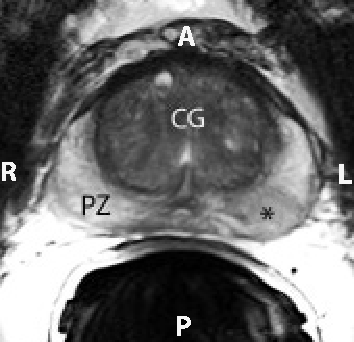
\includegraphics[width=0.3\linewidth]{figs/mr_anatomy/T2_base} \\
(a) MR T2WI Apex & (b) MR T2WI Mid-gland & (c) MR T2WI Base \\
\end{tabular}
\caption{Axial T2-weighted MR images of the prostate show the apex (a),
    mid-gland (b), and base (c).  The peripheral zone (PZ) is of higher signal
    intensity than the central gland (CG), the latter which is composed of the
    central zone and the transitional zone. The apex (a) is composed mostly of
    PZ glandular tissue and the urethra is seen at the level of the mid-gland as
    an inverted ``U'' (b). Note the area of hypointense signal in the
    peripheral zone at the mid-gland and base (asterisk, b and c), which
    represents a prostatic tumor.  The posterior (P) aspect of the prostate is
    adjacent to the endorectal coil, and the right (R)-to-left (L) extent of
    the prostate is referred to as the lateral-to-lateral axis in the subsequent
    analysis.}
\label{fig:mr_anatomy} 
\end{figure}


\begin{figure}[htb!]
\centering
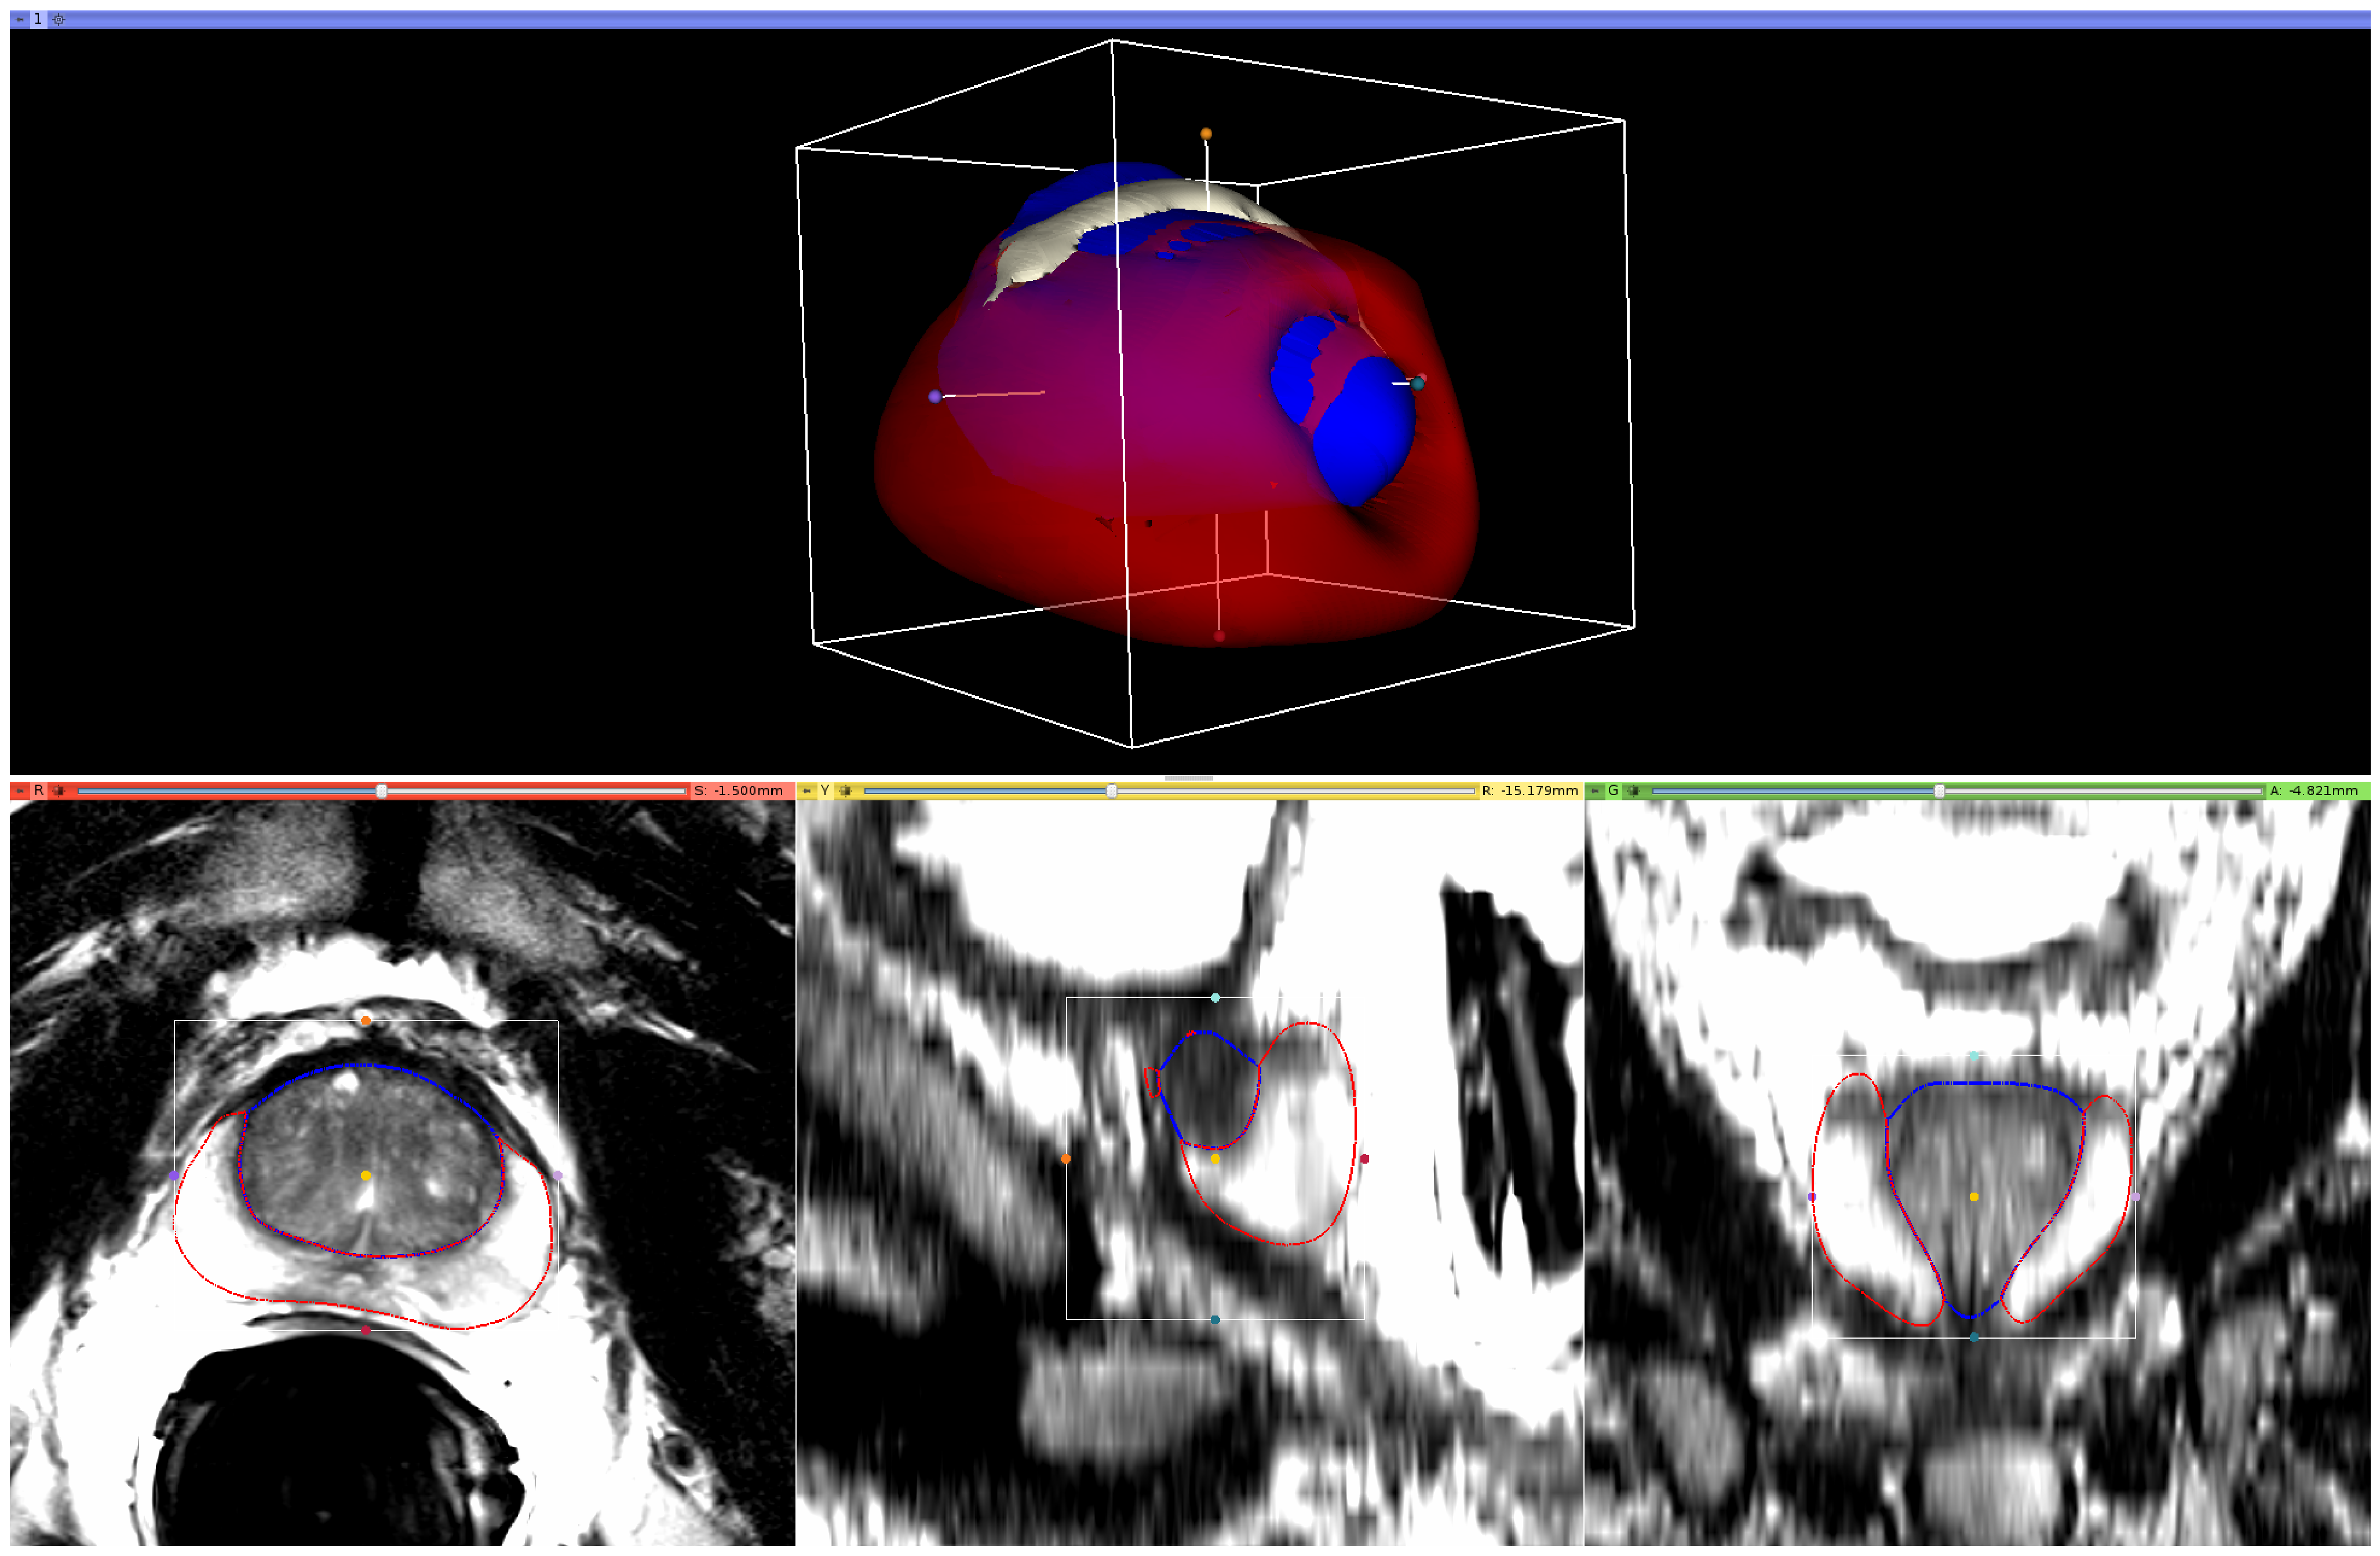
\includegraphics[width=1.0\textwidth]{figs/MR_P79_SegsVol.eps}
\caption{Representative MR T2WI segmentations and rendered volume performed in
    3D Slicer, with the peripheral zone (PZ) being delineated in red, the
    central gland (CG) being delineated in blue, and the anterior fibromuscular
    stroma (AFS) being shown in gray.  The AFS was combined with the PZ for
    quantitative analyses shown herein.  The native imaging plane for
    segmentation is the axial view, shown in the bottom left image.  The bottom
    middle and right images show the projections of the rendered model segment
    outlines in the sagital and coronal views, respectively.}
\label{fig:mr_segs_vol} 
\end{figure}


\subsubsection{Ultrasound Image Segmentation and Modeling}
Sagittal B-mode and ARFI ultrasound image stacks were segmented in 3D Slicer
using the \verb+draweffect+ tool to model and measure the prostate capsule and CG
volume and tri-axial dimensions.  The sagittal imaging plane was chosen for
segmentation because it has a greater number of easily identifiable anatomical
structures:  seminal vesicles in the left and right posterior base, urethra in
the mid apex, surrounding fibromuscular tissue in the anterior , and rectum in
the posterior  than either the axial or coronal views. Prostate capsule was
segmented in B-mode as this modality offers both high contrast between
prostatic tissue and surrounding periprostatic fat, and better SNR in the
anterior capsule region than ARFI images. ARFI was used to segment central gland as
there is clear delineation in this modality between central gland and
peripheral zone. This delineation is a result of the greater density of
connective tissue within the central gland versus the peripheral zone meaning
the central gland is stiffer than the surrounding peripheral zone.  Prior to
segmentation, both the B-mode and ARFI image stacks were downsampled along the
sagittal axis by a factor of 20 (i.e., from 360 slices per image stack to 18
slices per image stack). This was done because segmenting 360 slices per image
is inordinately time intensive, and does not improve the quality of the 3D
rendered model any more than segmenting the more reasonable 18 slices per image
stack. The parameters used for the resample scalar volume tool are shown below:

WHAT GOES HERE?

Although, segmentations were performed along the sagittal plane, label map
intersections in the axial and coronal views were used during active creation
of the sagittal segmentation to further improve segmentation accuracy.  This
was done by using the resampled image stack, B-mode for capsule and ARFI for
CG, as the background in the sagittal plane, and the original image stack as
background in the axial and coronal planes. All three orthogonal views were set
to the label map assigned to the resampled volume. The B-mode derived capsule
was segmented and modeled before the central gland. Parameters used for 3D
model rendering were identical to those used in table X for MR modeling. The
modeled capsule  helprf guide the CG segmentation by enabling capsule model
intersections in the three orthogonal planes during CG segmentation. The
capsule provided an outer boundary for the CG segmentation. The capsule and CG
models were then measured identically to the MR measurement procedure.

\begin{figure}[htb!]
\centering
\begin{tabular}{c}
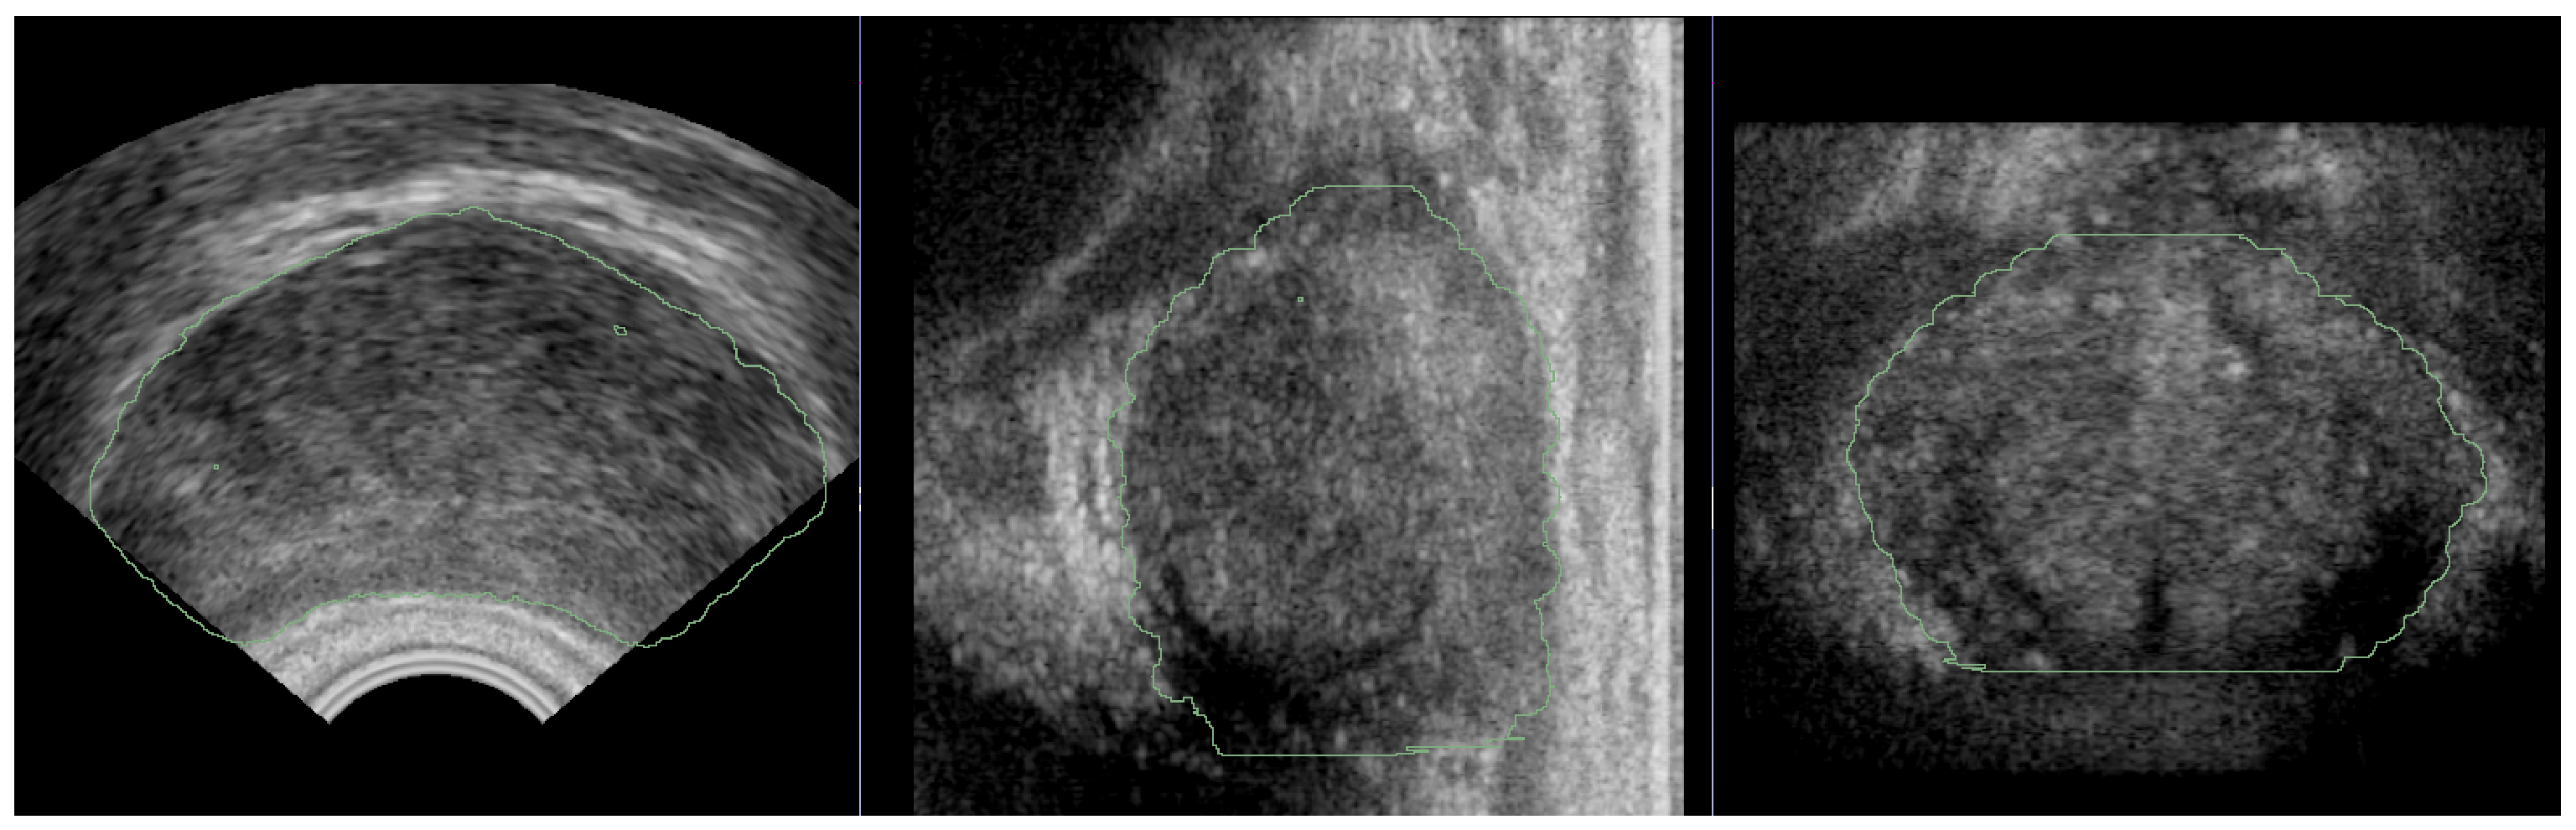
\includegraphics[width=1.0\textwidth]{figs/Bmode_CapsuleSegs.eps} \\
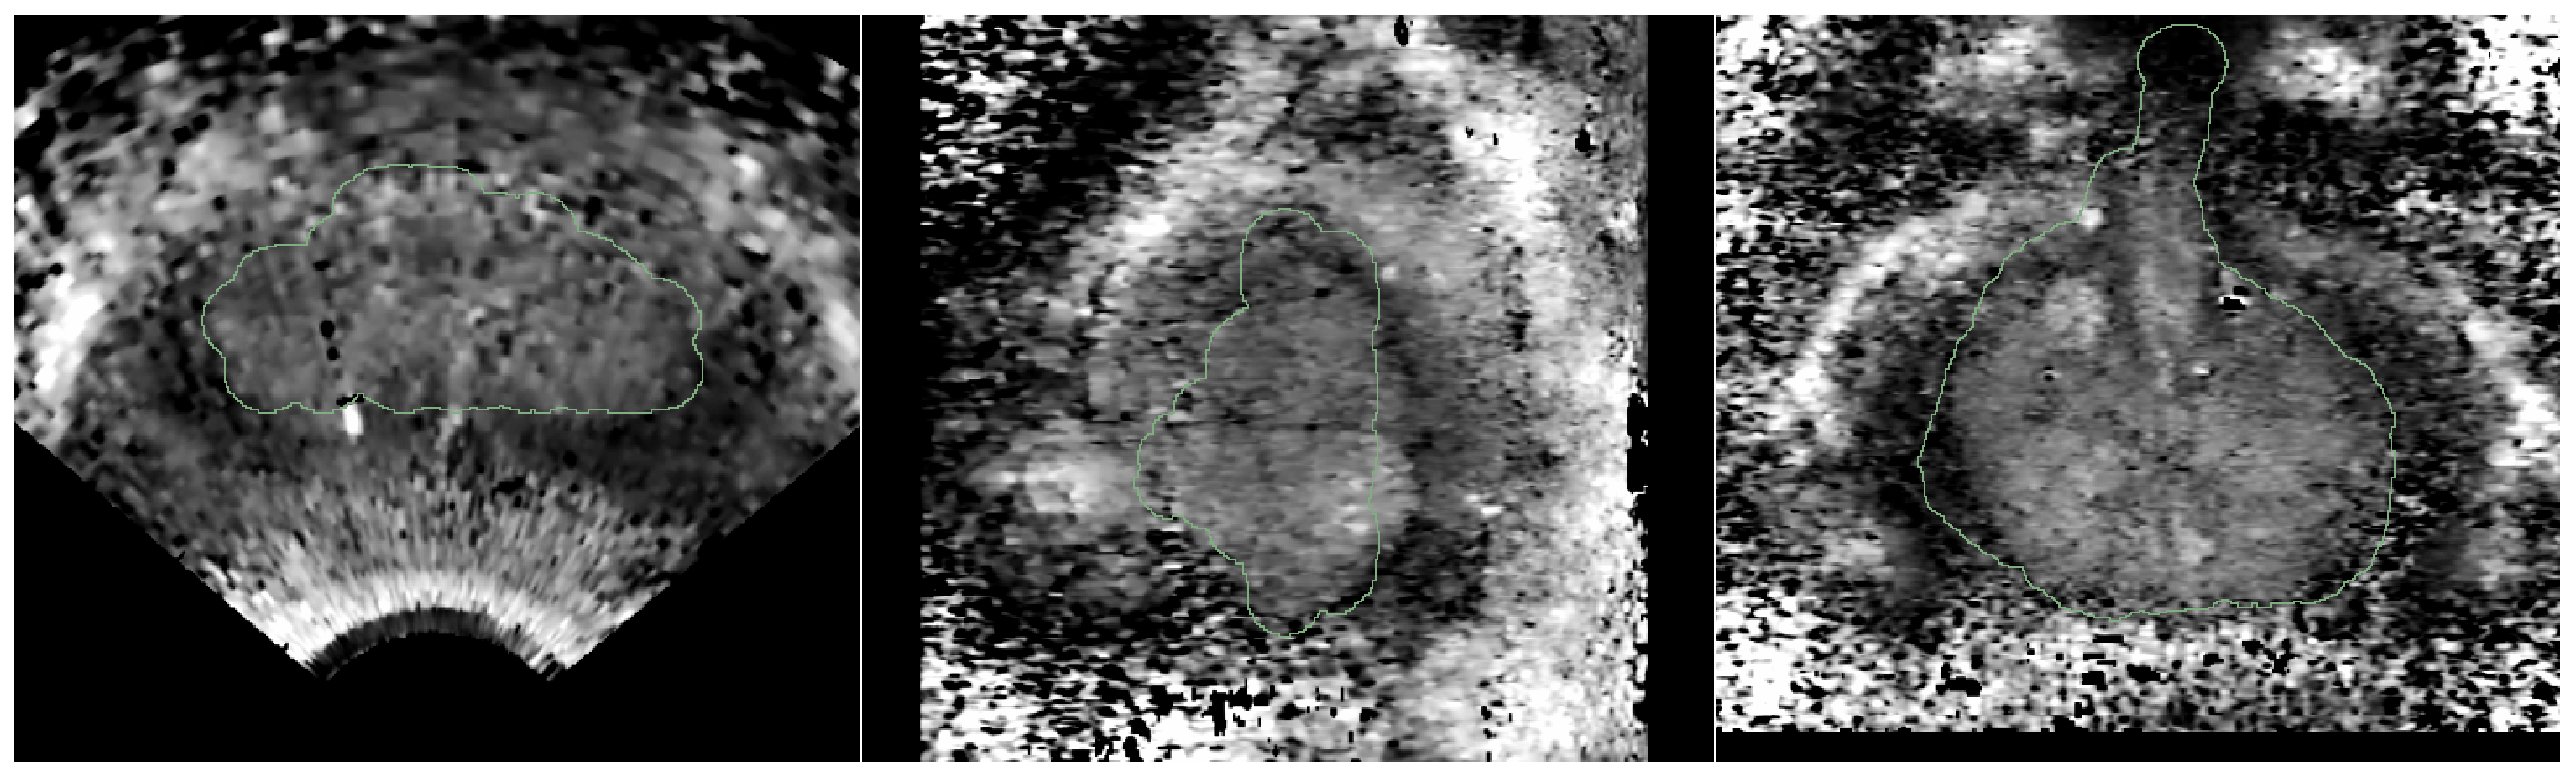
\includegraphics[width=1.0\textwidth]{figs/ARFI_CGsegs.eps} \\
\end{tabular}
\caption{Representative B-mode (top row) and ARFI images (bottom row), with
    superimposed segmentation outlines of the capsule and CG, respectively, for
    the same study subject shown in Figure~\ref{fig:mr_segs_vol}.  The B-mode
    images were segmented in the axial view, using the hypoechoic border of the
    capsule.  Notice that for large prostates, like the one shown in this
    figure, that the edges of the organ were not always captured in the imaging
    field-of-view.  The CG in the ARFI images was typically segmented using the
    coronal view, which, especially in the presence of extensive BPH, can have
    a very characteristic, heterogeneous appearance.  It should be noted that
    the coronal views in these ultrasound images are flipped 180\degree relative
    to the same images in Figure~\ref{fig:mr_segs_vol}.}
\label{fig:arfi_segs} 
\end{figure}


\begin{figure}
\centering
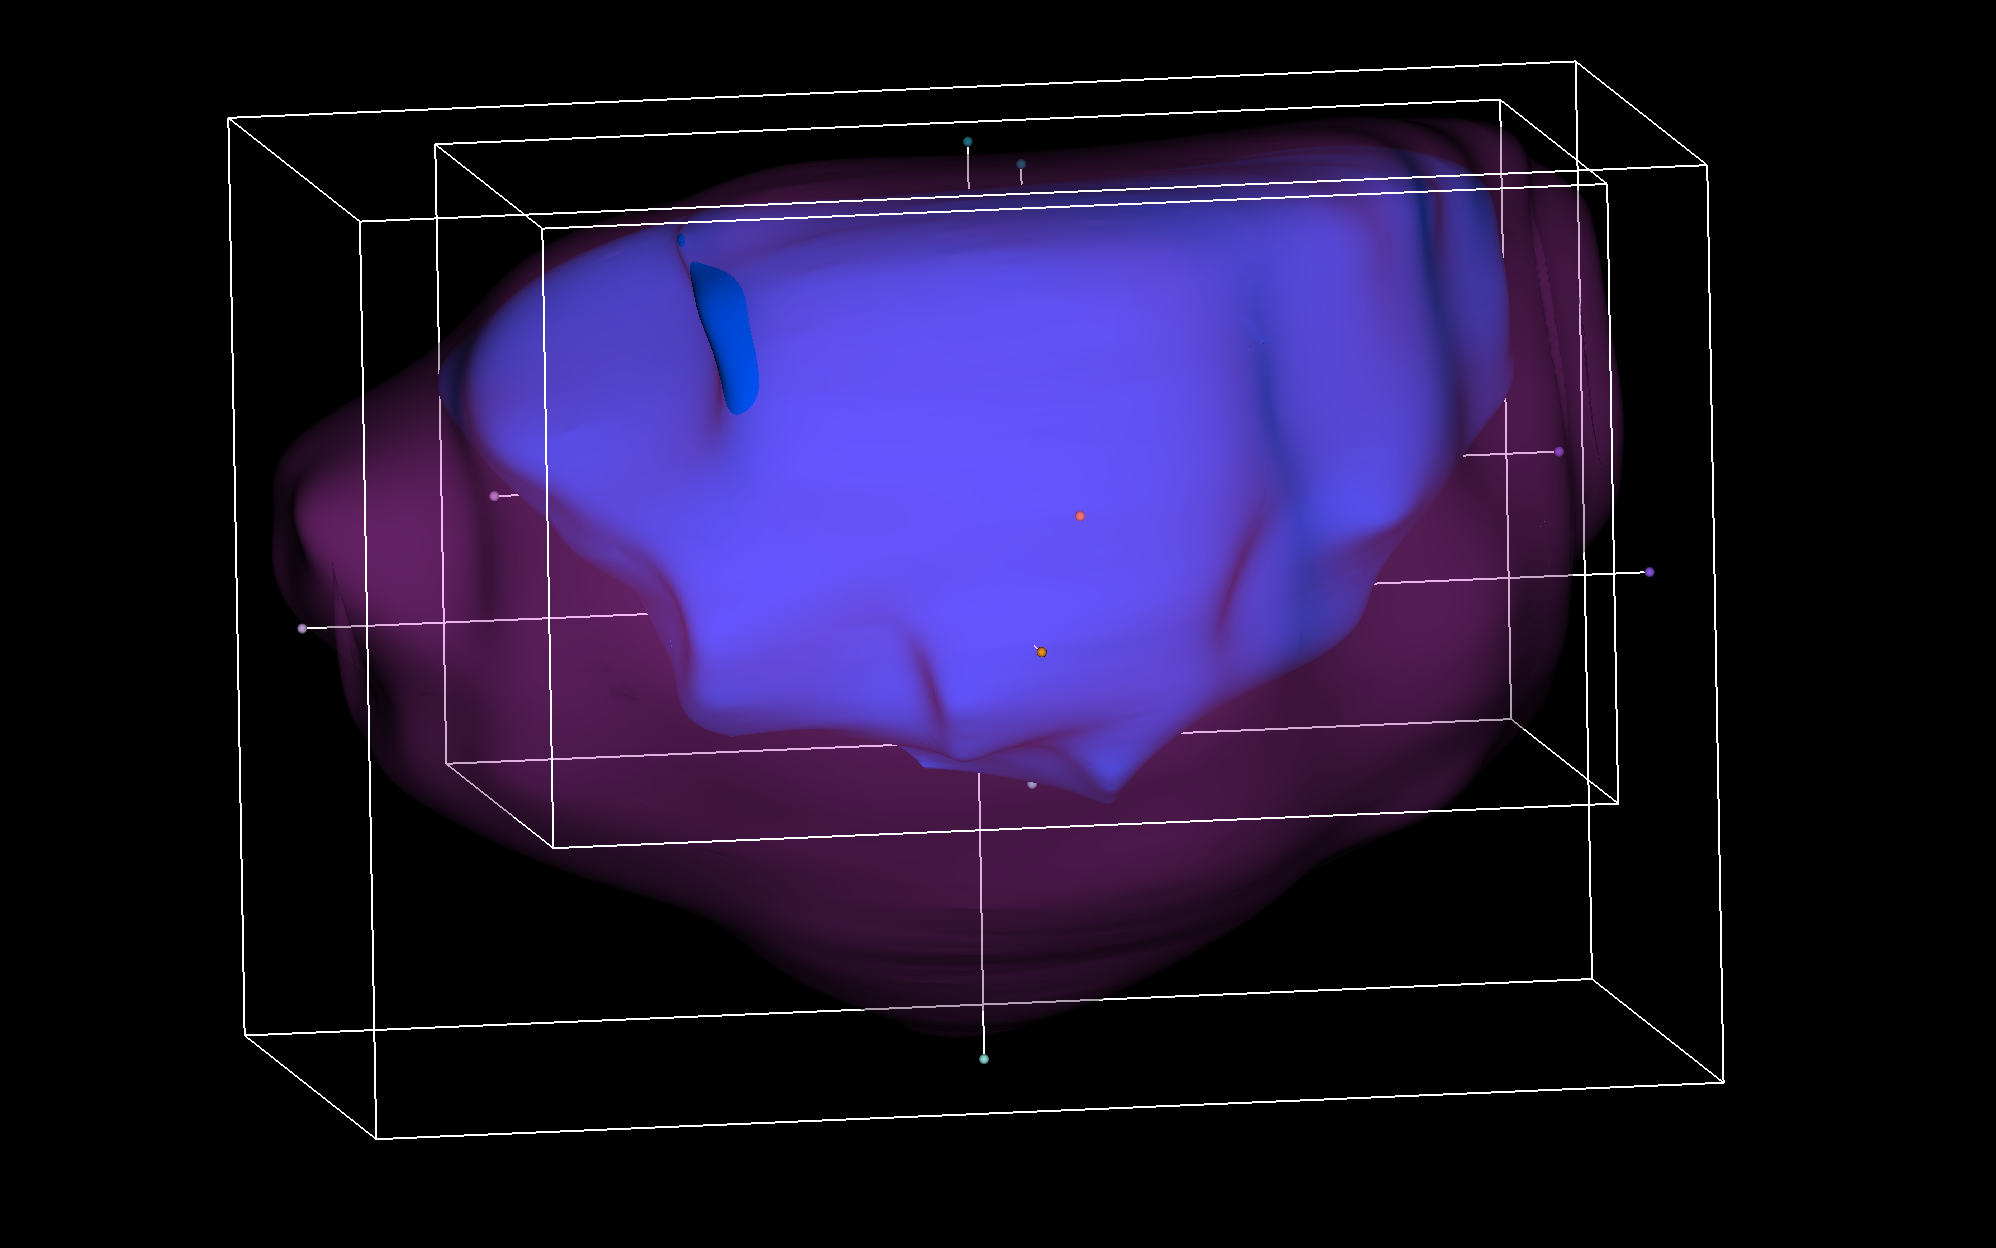
\includegraphics[width=0.5\textwidth]{tyler/ROI_methods.png}
\caption{An example of the 3D Slicer ROI tool surrounding the prostate capsule (magenta)
    and central gland (blue) of study subject. This ROI tool is used to find the
    tri-axial dimensions of the prostate, in both the ultrasound and MR image
    datasets.}
\label{fig:roi_tool} 
\end{figure}

